\nonstopmode

\documentclass[letterpaper,11pt,titlepage]{article}
\usepackage{amsthm,amssymb,mathtools}
\mathtoolsset{showonlyrefs}
\usepackage{bm}
\usepackage[margin=1in]{geometry}
\usepackage{booktabs}
\usepackage{enumitem}
\usepackage{framed}
\usepackage{tikz}
\usetikzlibrary{shapes,arrows.meta,positioning,patterns,calc}
\usepackage{pgfplots}
\pgfplotsset{compat=1.9}
\usepackage{listings}
%\usepackage[numbered,framed]{mcode}

\usepackage{algpseudocode}
\usepackage{algorithm}

\usepackage{fancyhdr}
\pagestyle{fancy}
\fancyhead{}
\fancyfoot{}
\fancyfoot[L]{K.\ Okkelberg}
\fancyfoot[R]{\thepage}
\renewcommand{\headrulewidth}{0pt}
\renewcommand{\footrulewidth}{0.5pt}

\newcommand*\dif{\mathop{}\!\mathrm{d}}
\newcommand{\trans}{^\text{T}}
\newcommand{\herm}{^\text{H}}
\DeclareMathOperator{\E}{E}
\DeclareMathOperator{\trace}{trace}
\DeclareMathOperator{\sign}{sign}
\DeclareMathOperator{\eig}{eig}
\let\Pr\relax
\DeclareMathOperator{\Pr}{P}
\newcommand*\pder[2]{\frac{\partial #1}{\partial #2}}
\newcommand*\der[2]{\frac{\dif #1}{\dif #2}}
\newcommand*\R{\mathbb{R}}

\renewcommand\qedsymbol{$\blacksquare$}

\tikzstyle{line} = [draw,>=latex]
\tikzstyle{dot} = [circle,fill=black,inner sep=0pt,minimum size=4pt]

\begin{document}

\title{ECE 6553: Homework \#5}
\author{Klaus Okkelberg}
\date{April 18, 2017}
\maketitle

\setlist{listparindent=\parindent}

\begin{enumerate}[leftmargin=0pt]

    \item 
        \begin{enumerate}
            \item \begin{itemize}
                \item We need $R=R\trans\succ 0$ so that the cost term $u\trans Ru$ is non-negative (so cost can't go to negative infinity) and that the term is zero if and only if $u=0$ (so the control can't be infinite and while having zero cost).
                \item We need $Q=Q\trans\succcurlyeq 0$ and $S=S\trans\succcurlyeq 0$ so the terms $x\trans Qx$ and $x\trans(T)Sx(T)$ are non-negative (so cost can't go to negative infinity).
                    \item There are no conditions on $A$ and $B$ since this is a finite-horizon problem. The observability and controllability of the system does not matter since the cost and the norm of the state are guaranteed to be finite (unless the initial state has infinite norm) with the finite terminal time.
                \end{itemize}

            \item \begin{itemize}
                \item We need $R=R\trans\succ 0$ and $Q=Q\trans\succcurlyeq 0$ for the same reasons as in the previous question.
                \item We need $(A,B)$ to be completely controllable so that there exists $u$ such that $x\to0$ as $t\to\infty$ (so the cost is finite). Specifically, completely controllable means that there exists $u$ that takes the system between any two points.
                \item We need $(A,\sqrt{Q})$ to be completely observable so that, over time, $x$ affects $x\trans Qx$, meaning that $\Vert x\Vert\to\infty$ results in infinite cost.
            \end{itemize}

            \item Assume that a solution to the Riccati equation exists. We will show it has to be symmetric. First, note that $S$ is symmetric so $P(T)=S=S\trans=P\trans(T)$. Furthermore, by symmetry of $Q$ and $R$,
                \begin{align}
                    \dot P\trans &= -[A\trans P]\trans - [PA]\trans - Q\trans + [PBR^{-1}B\trans P]\trans \\
                                    &= -P\trans A - A\trans P\trans - Q + P\trans B R^{-1} B\trans P\trans
                \end{align}
                Therefore, for symmetric $P(t)$, $\dot P(t)$ is also symmetric. Furthermore, since the boundary value $P(T)$ is symmetric, the solution $P(t)$ will stay in the set of symmetric matrices, i.e.\ $P(t)=P\trans(t)\ \forall t\in[0,T]$.
                
                %Assume that the proposition $P(t)=P\trans(t)\ \forall t$ is not true. Then, there exist $t\in\Theta$ such that $P(t)\neq P\trans(t)$. Let $\tau=\max\Theta$. The maximum exists because
                %
                %Note that $\tau<T$ because $P(T)=P\trans(T)$, so $P(t)=P\trans(t)$ for $t\in(\tau,T]$. Then,
                %\begin{gather}
                    %P(\tau) = P(T) - \int_\tau^T \dot P(t) \dif t = P\trans(T) - \int_\tau^T \dot P\trans(t) \dif t = \left[ P(T) - \int_\tau^T \dot P(t) \dif t \right]\trans = P\trans(\tau),
                %\end{gather}
                %and we have a contradiction. Therefore, the propsition is true, i.e.\ $P(t)=P\trans(t)\ \forall t\in[0,T]$. \qed
        \end{enumerate}

    \item For the claimed solution to be the optimal solution, it has to satisfy the HJB equation
        \begin{gather}
            -\pder{J^*}{t} = \min_u \left\{ \frac12 \rho\big[x(t)-\sigma(t)\big]^2 + \frac12 u^2(t) + \pder{J^*}{x} \big[ax(t) + bu(t)\big] \right\},
        \end{gather}
        where $J^*(x,T)=\Psi(x(T))=0$. Assume that the form of the optimal cost-to-go is correct. We start by minimizing the RHS with respect to $u$:
        \begin{align}
            \pder{\{\cdot\}}{u} &= u + b\pder{J^*}{x} = 0 \\
            u &= -b \pder{J^*}{x} = -b \pder{}{x} \left[ \frac12 x^2(t) p(t) + w(t) x(t) + v(t) \right] \\
            u &= -b \big[ p(t) x(t) + w(t) \big] \label{eq:p2_u}
        \end{align}
        Substituting the optimal $u$ into the HJB equation produces
        \begin{gather}
            -\pder{J^*}{t} = \frac12 \rho (x-\sigma)^2 + \frac12 b^2 (px+w)^2 + (px+w)[ax-b^2(px+w)] \\
            \begin{aligned}
                -\pder{}{t}\left[ \frac12 x^2(t) p(t) + w(t) x(t) + v(t) \right] &= \frac12 \rho (x^2-2x\sigma+\sigma^2) + \frac12 b^2(p^2x^2 + 2pwx + w^2) \\
                                                                                 & \qquad {} + (a-b^2p)px^2 + [-b^2pw+(a-b^2p)w]x - b^2w^2
            \end{aligned} \\
            \begin{aligned}
                - \frac12 \dot p x^2 - \dot w x - \dot v &= \frac12 \Big[\rho+b^2p^2+2(a-b^2p)p\Big] x^2 + \Big[-\rho\sigma + b^2pw - 2b^2pw + aw\Big] x \\
                                                         & \qquad {} + \frac12 \rho\sigma^2 + \frac12 b^2w^2 - b^2w^2 \\
                \frac12 \dot p x^2 + \dot w x + \dot v &= \frac12 \Big(-\rho -2ap +b^2p^2\Big) x^2 + \Big(\rho\sigma - aw + b^2pw \Big) x - \frac12 \rho\sigma^2 + \frac12 b^2w^2
            \end{aligned}
        \end{gather}
        Equating like powers of $x$, we find
        \begin{align}
            \dot p &= -2ap + p^2b^2 - \rho \label{eq:p2_p} \\
            \dot w &= -(a-b^2p)w + \rho\sigma \label{eq:p2_w} \\
            \dot v &= \frac12 \big( w^2b^2 - \sigma^2\rho \big) \label{eq:p2_v}
        \end{align}
        Furthermore, since $J^*(x,T)=0\ \forall x$, we need 
        \begin{gather}
            p(T)=w(T)=v(T)=0. \label{eq:p2_term}
        \end{gather}
        Since equations \eqref{eq:p2_u}, \eqref{eq:p2_p}, \eqref{eq:p2_w}, \eqref{eq:p2_v}, and \eqref{eq:p2_term} match the claimed solution, it is indeed the optimal solution. \qed

    \item 
        \begin{enumerate}
            \item Note that $x\in\R^5$ since $A$ is $5\times 5$. In Matlab, we can see that the controllability matrix has full rank (\texttt{rank(ctrb(A,B)) = 5}). This means the system is completely controllable.

                For the uncontrolled system, using Matlab we find the eigenvalues of $A$ are
                    \begin{gather}
                        \eig(A) = 
                        \begin{bmatrix*}[r]
                            -24.1755 \\
                            -16.4772 \\
                            -5.4012 \\
                            20.0907 \\
                            15.3074
                        \end{bmatrix*}
                    \end{gather}
                    Since there are positive eigenvalues, the uncontrolled system $\dot x=Ax$ is unstable.
                \item I set $Q=qI$ and $R=I$, where $q>0$, and varied $q$. I tried $q$ in the form of $10^{k}$, $k\in\mathbb Z$. I found that $k\le 4$ produced similar shapes for $x$ and $u$; for increasing $k$, $x$ converges slightly faster to 0 and initial $u$ is slightly larger, see Figs.~\ref{fig:p3_-4} and \ref{fig:p3_4}. For $k\ge 5$, $x$ converges at about the same rate but the initial $u$ is significantly increased from $k<5$, see Figs.~\ref{fig:p3_5} and \ref{fig:p3_6}.

                    Based on these findings, I choose
                    \begin{gather}
                        Q=10^4 I, \quad R=I,
                    \end{gather}
                    because this has the best trade-off between fast convergence of $x$ without expending too much control energy $\Vert u\Vert^2$.

                    \begin{figure}
                        \centering
                        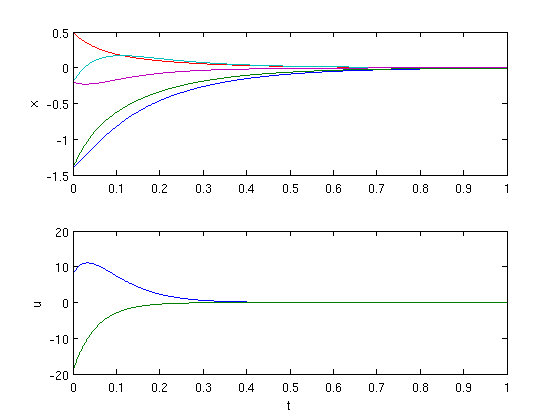
\includegraphics[width=0.8\textwidth]{hw5p3_-4}
                        \caption{$Q=10^{-4} I$, $R=I$}
                        \label{fig:p3_-4}
                    \end{figure}
                    \begin{figure}
                        \centering
                        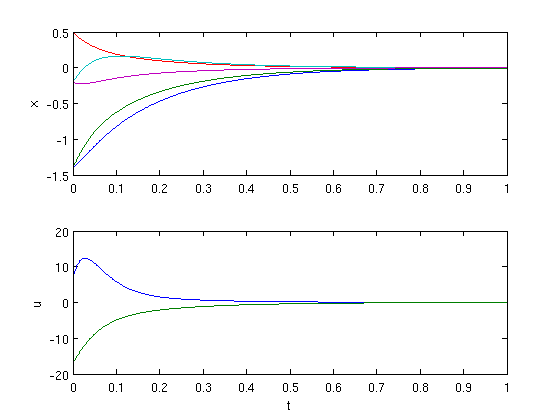
\includegraphics[width=0.8\textwidth]{hw5p3_4}
                        \caption{$Q=10^{4} I$, $R=I$}
                        \label{fig:p3_4}
                    \end{figure}
                    \begin{figure}
                        \centering
                        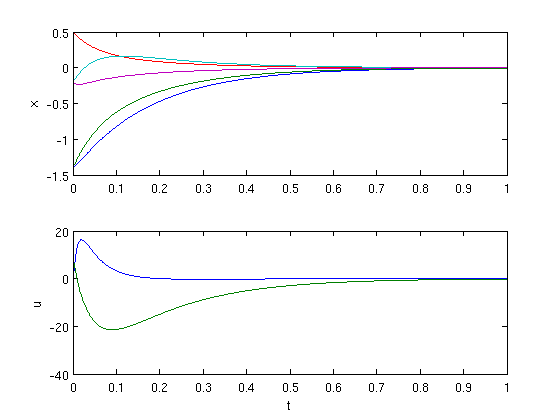
\includegraphics[width=0.8\textwidth]{hw5p3_5}
                        \caption{$Q=10^{5} I$, $R=I$}
                        \label{fig:p3_5}
                    \end{figure}
                    \begin{figure}
                        \centering
                        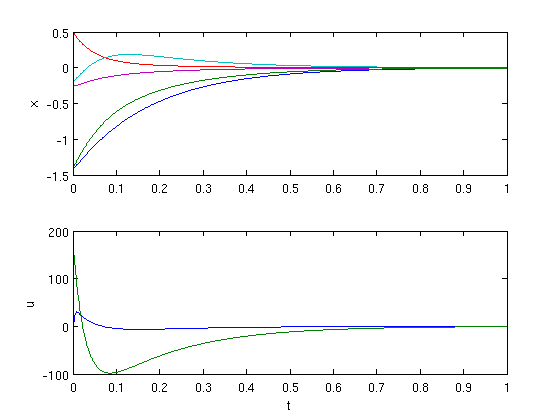
\includegraphics[width=0.8\textwidth]{hw5p3_6}
                        \caption{$Q=10^{6} I$, $R=I$}
                        \label{fig:p3_6}
                    \end{figure}
        \end{enumerate}

        \clearpage

    \item 
        \begin{enumerate}
            \item For this problem, we have
                \begin{gather}
                    Q = \begin{bmatrix}
                        1 & 1 \\ 1 & 1
                    \end{bmatrix},\
                    R = 1,\
                    A = \begin{bmatrix}
                        1 & 1 \\ -1 & 0
                    \end{bmatrix},\
                    B = \begin{bmatrix}
                        0 \\ 1
                    \end{bmatrix}.
                \end{gather}
                We have $\eig(Q)=0,2$ and $\eig(R)=1$, so $Q\succcurlyeq 0$ and $R\succ 0$. Additionally,
                \begin{gather}
                    \sqrt{Q} = \frac{1}{\sqrt{2}} Q.
                \end{gather}
                The controllability matrix is
                \begin{gather}
                    \Gamma = \begin{bmatrix}
                        B & AB
                    \end{bmatrix}
                    = \begin{bmatrix}
                        0 & 1 \\ 1 & 0
                    \end{bmatrix}
                \end{gather}
                with rank 2, so the system is completely controllable. Furthermore, the observability matrix is
                \begin{gather}
                    \Omega = \begin{bmatrix}
                        \sqrt{Q} \\ \sqrt{Q} A
                    \end{bmatrix}
                    = \begin{bmatrix}
                        1/\sqrt{2} & 1/\sqrt{2} \\
                        1/\sqrt{2} & 1/\sqrt{2} \\
                        0 & 1/\sqrt{2} \\
                        0 & 1/\sqrt{2}
                    \end{bmatrix}
                \end{gather}
                with rank 2, so the system is completely observable. Since all the conditions for infinite-horizon LQ are met, the problem is well-defined.
            \item In Matlab, \texttt{care(A,B,Q,R)} produces
                \begin{gather}
                    P = \begin{bmatrix}
                        4.8284 & 2.4142 \\
                        2.4142 & 2.4142
                    \end{bmatrix}.
                \end{gather}
                The optimal controller is given by
                \begin{gather}
                    u = -R^{-1} B\trans P x
                    = -1^{-1} \times \begin{bmatrix}
                        0 & 1
                    \end{bmatrix} \times
                    \begin{bmatrix}
                        4.8284 & 2.4142 \\
                        2.4142 & 2.4142
                    \end{bmatrix} x
                    = \boxed{- \begin{bmatrix}
                        2.4142 & 2.4142
                    \end{bmatrix} x }
                \end{gather}
        \end{enumerate}

    \item Note that by the chain rule
        \begin{gather}
            \der{}{t} \Big[ e^{A\trans t} Q e^{At} \Big] = \der{e^{A\trans t}}{t} Q e^{At} + e^{A\trans t} Q \der{e^{At}}{t} = A\trans e^{A\trans t} Q e^{At} + e^{A\trans t} Q e^{At} A.
        \end{gather}
        Additionally, for asymptotically stable $\dot x=Ax$
        \begin{gather}
            \lim_{t\to\infty} e^{At} = \lim_{t\to\infty} e^{A\trans t} = 0.
        \end{gather}
        Substituting the proposed solution into the ARE produces
        \begin{align}
            0 &= A\trans P + PA + Q \\
              &= A\trans \int_0^\infty\! e^{A\trans t} Q e^{At} \dif t + \int_0^\infty\! e^{A\trans t} Q e^{At} \dif t \times A + Q \\
              &= \int_0^\infty\! \Big[ A\trans e^{A\trans t} Q e^{At} + e^{A\trans t} Q e^{At} A \Big] \dif t + Q \\
              &= \int_0^\infty\! \der{}{t} \Big[ e^{A\trans t} Q e^{At} \Big] \dif t + Q \\
              &= \Big[ e^{A\trans t} Q e^{At} \Big]_0^\infty + Q \\
              &= 0\times Q\times 0 - I\times Q\times I + Q = -Q + Q = 0 \qed
        \end{align}

    \item There were 24 questions.

\end{enumerate}

\end{document}
